\part{Background on the immersed interface method}
\section{Introduction to the immersed interface method}
The IIM stemmed from a need to accommodate discontinuities in solutions or coefficients more generally than with the previously popular Immersed Boundary Method \cite{levequeli94}.
The Immersed Boundary Method was developed initially in \cite{viecelli69} and \cite{viecelli71} as an extension to the Marker and Cell computational fluid dynamics technique \cite{welch66}.
The MAC method was capable of simulating fluid flow around rigid boundaries by dividing the domain into a rectangular mesh, however it could not accommodate moving boundaries that deformed during the simulation of the flow.
The method employed by Viecelli was popularized by Peskin in his papers modelling the flow of blood in the heart (\cite{peskin72} and \cite{peskin77}) and named the Immersed Boundary Method (IB).
The IB method models the boundaries as fluid particles which move with the local velocity of the fluid, but exert a force on the surrounding fluid. This force at the boundary is modeled as a smoothed Dirac delta function \cite{peskin02}, but this leads to the interface being 'smeared' up to the grid size.
Although the immersed boundary method is still used in many fields, (particularly in Peskin's field of bio-mechanics eg. \cite{heys07}, \cite{yakhot05}) the IIM has some advantages over the immersed boundary method.

The IIM was first developed and outlined in a thesis by Li in 1994 \cite{li94} and a paper based on this work by Leveque and Li \cite{levequeli94}.
These papers develop the IIM for general one and two dimensional elliptic problems and heat equation problems, with both stationary and moving interfaces.
A key advantage of the IIM is that it exactly enforces discontinuities in parameters or the solution and its derivatives across boundaries, where as Peskin's method smooths these discontinuities in order to model them.
The smoothing is accomplished by introducing a discrete delta function that approximates any singularities.
However the accuracy of this method is limited by the size of the grid.
In contrast to the IB method, the IIM attempts to correct the solution only at the discontinuity, and does so in a way which is independent of the grid.
The result of this is that the IIM accurately preserves sharp boundaries where as the IB method does not.
This can be seen clearly in figure \ref{fig:one}.

\begin{figure}[b]
    \centerline{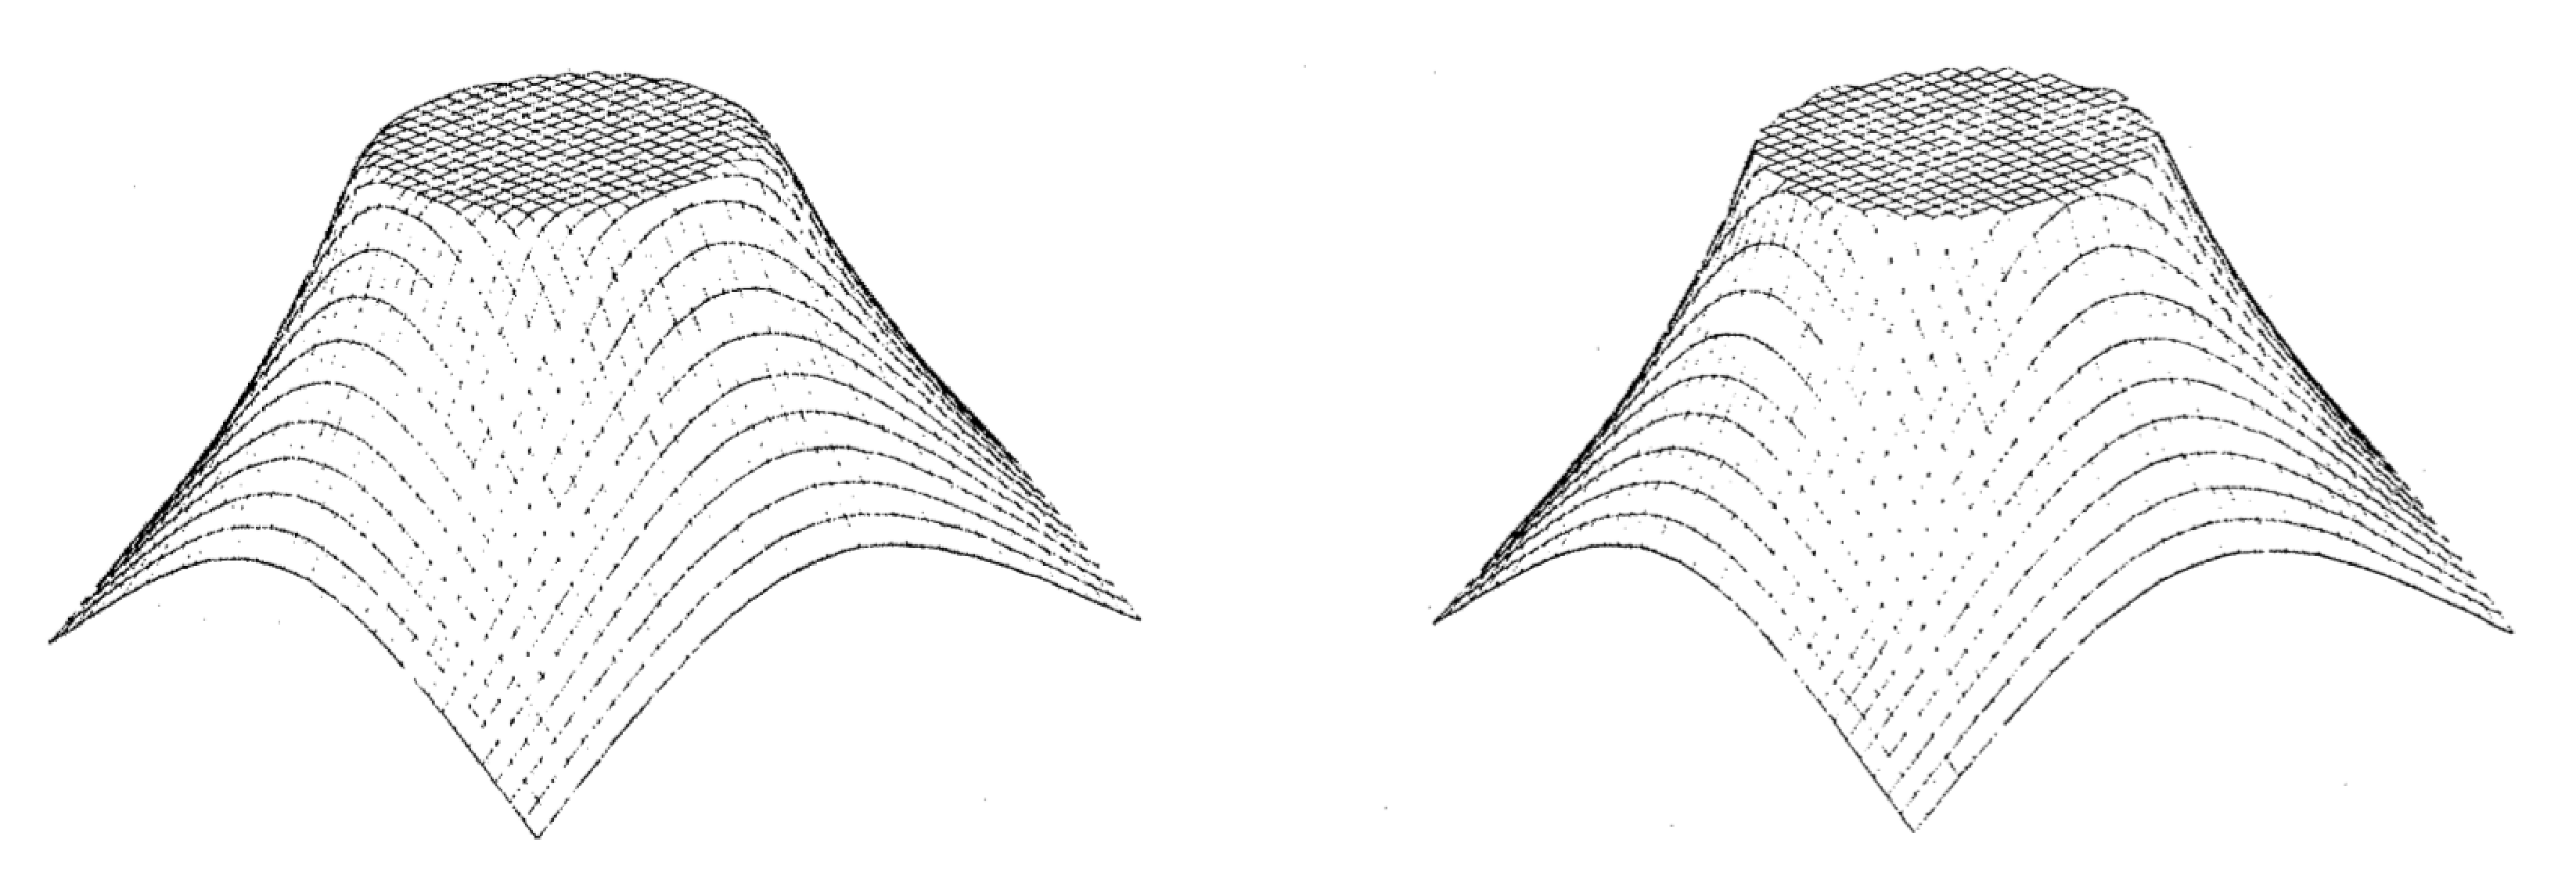
\includegraphics[width=0.8\textwidth]{diagrams/LevequeLiComparison.eps}}
    \vskip0.5cm
    \caption{Solution to an elliptic interface problem using (a) a discrete delta function such as in Peskin's method and (b) the IIM. Note that discontinuity is much sharper when using the IIM. Figure from \cite{levequeli94}}
    \label{fig:one}
\end{figure}

Another advantage of the IIM is that it allows for discontinuities in any parameter, as well as discontinuities that must be enforced in the solution and its derivatives. 
This allows for a much wider variety in the problems that can be solved using the IIM.

This introductory part will be organized into four sections.
The first section will briefly introduce the IIM in 1D and provide an example of how the IIM works.
The second section will discuss the problems and solutions associated with applying the IIM to parabolic, elliptic and hyperbolic PDEs.
The third section will discuss some augmentations and modifications to the IIM. 
The fourth section will provide some novel examples of how the IIM has been used to solve a range of problems.
